\section{Study Results}
\label{sec:eval}

\begin{figure}[ht]
    \centering
    \includegraphics[width=0.5\textwidth]{gfx/figures/distribution-unsafe-types.png}
    \caption{Distribution of different types of unsafe token types. Answers \ref{rq:distTypes}}
    \label{fig:unsafe-tokens-distribution}
\end{figure}

\begin{figure*}[ht]
    \centering
    {\scriptsize \includegraphics[width=\textwidth,height=6cm]{gfx/figures/unsafe-import-depth.tikz}}
    \caption{Import Depth of Unsafe Packages. Answers \ref{rq:depsDepth}: unsafe packages are around \checkNum{3.5 $\pm 2$} hops away, thus manageable to find manually. \jl{Add mean and deviation}}
    \label{fig:unsafe-import-depth}
\end{figure*}

\begin{figure*}[ht]
    \centering
    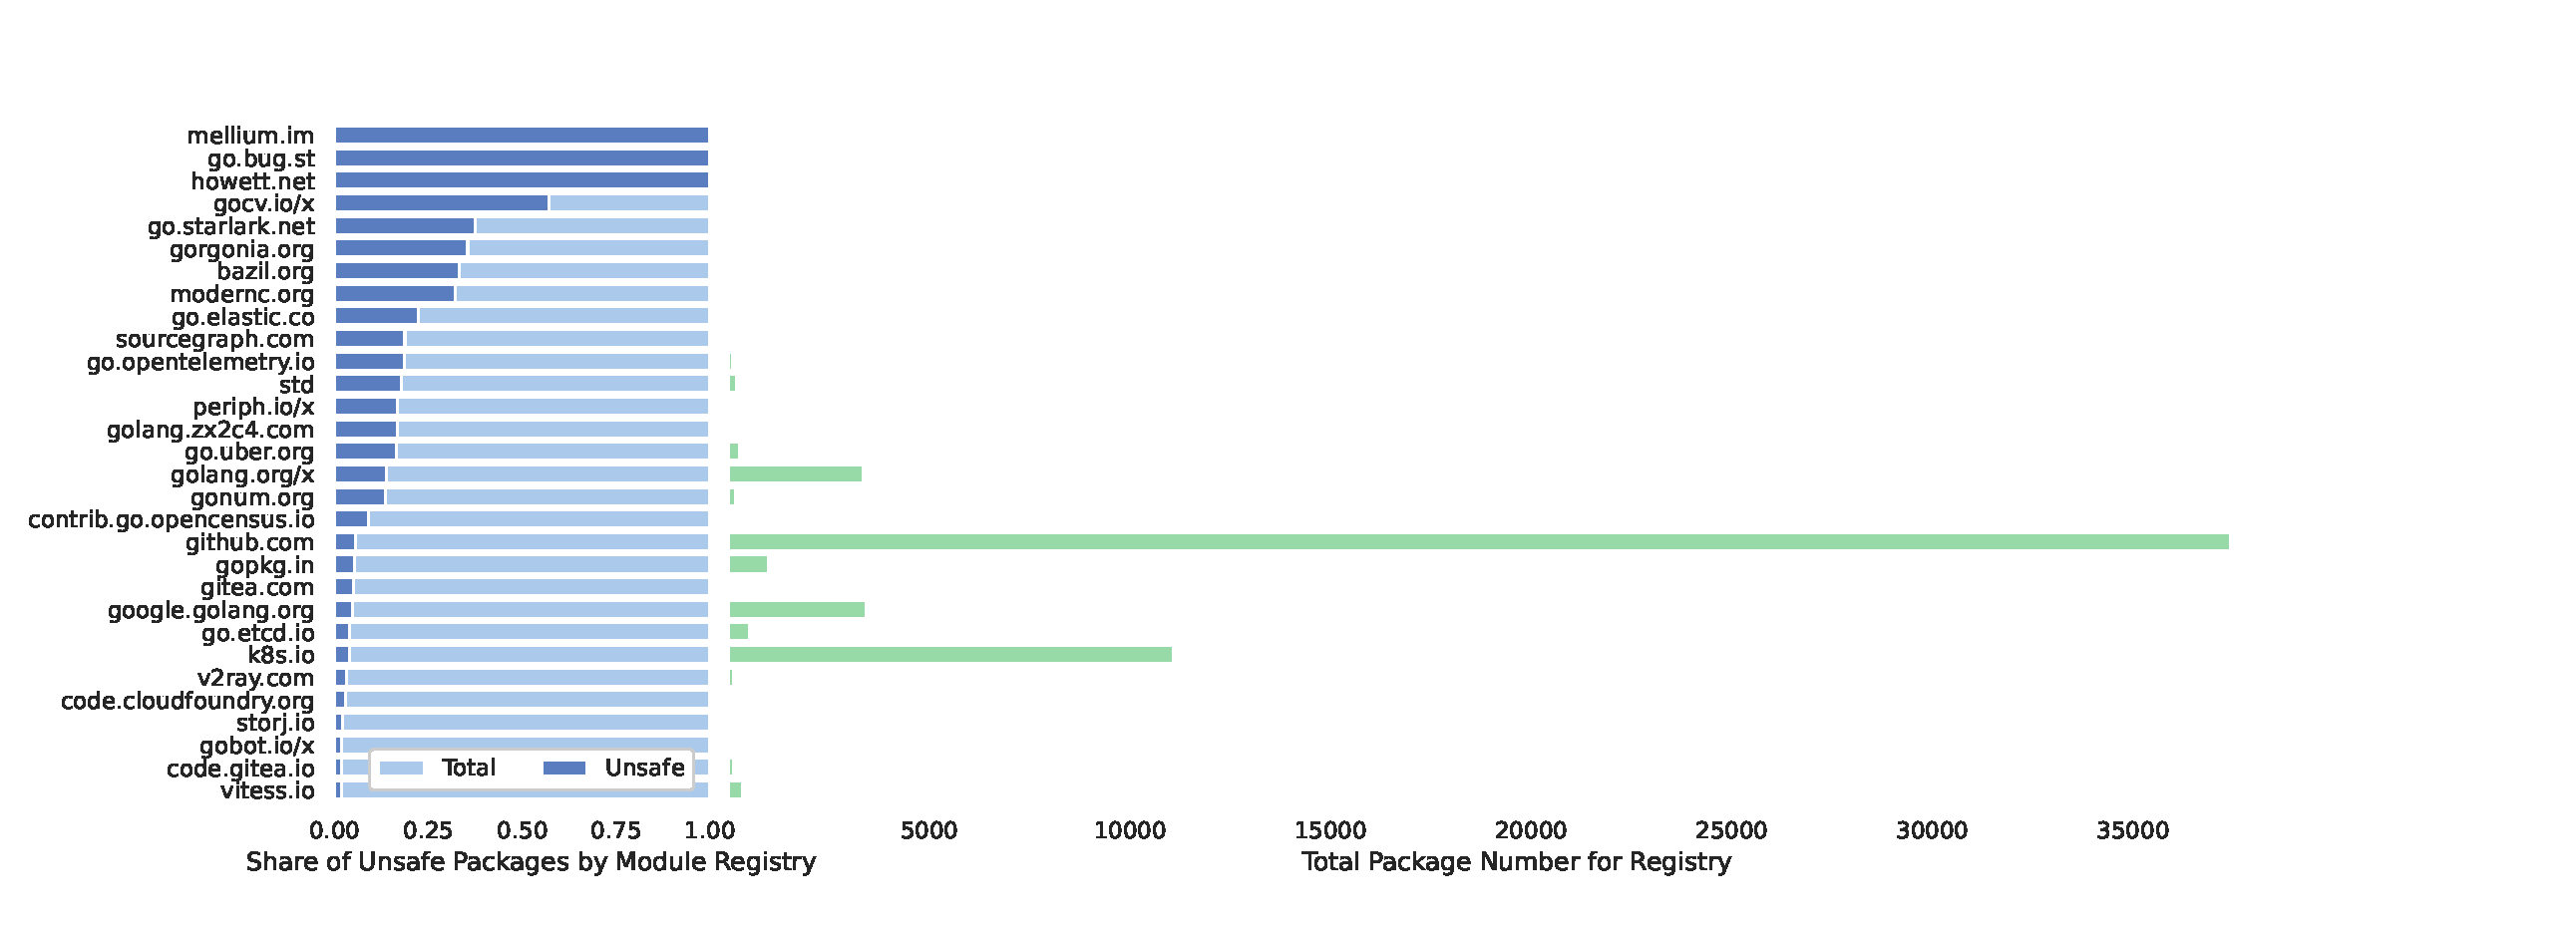
\includegraphics[width=\textwidth]{gfx/figures/unsafe-packages-by-registry-n30.eps}
    \caption{Share of Unsafe Packages by Registry along with Total Package Count for Registries, Showing the Top \checkNum{30} Registries by Unsafe Share. Answers \ref{rq:prevalDeps} in its current form}
    \label{fig:unsafe-by-registry}
\end{figure*}

\begin{table}[h]
    \centering
    \caption{Selected projects for creation of the labeled data set}
    \label{tbl:dataset-projects}
    \begin{tabular}{llrrll}
    \hline
        {}  &                                               Name &  Stars &  Forks &   Revision \\ \hline
        1   &                              kubernetes/kubernetes &  66512 &  23806 &  fb9e1946b0 \\
        2   &                       mattermost/mattermost-server &  18277 &   4157 &  e83cc7357c \\
        3   &                                    rancher/rancher &  14344 &   1758 &  56a464049e \\
        4   &                                   weaveworks/scope &   4354 &    554 &  bf90d56f0c \\
        5   &                                          rook/rook &   7208 &   1472 &  ff90fa7098 \\
        6   &                                      elastic/beats &   8852 &   3207 &  df6f2169c5 \\
        7   &                                hashicorp/terraform &  22151 &   5729 &  01f91316da \\
        8   &                                      cilium/cilium &   5501 &    626 &  9b0ae85b5f \\
        9   &                                       grafana/loki &   9537 &    922 &  10a1f28a85 \\
        10  &                                  gorgonia/gorgonia &   3373 &    301 &  5fb5944d4a \\
        \hline
    \end{tabular}
\end{table}

\begin{table*}[t]
    \centering
    \caption[Labeled unsafe.Pointer usages in application code samples Answers \ref{rq:purpose}]%
    {Labeled unsafe.Pointer usages in application code samples \newline \tiny ~ \newline \small
        \underline{eff}: efficiency, \underline{gen}: generics, \underline{ser}: (de)serialization,
        \underline{inev}: inevitable use, \underline{SR}: safer reflections, \underline{LC}: layout control,
        \underline{EA}: hide from escape analysis, \underline{UU}: unused,
        \underline{doc}: documentation \newline \tiny ~}
    \label{tbl:dataset-classes-app}
    \begin{tabular}{r|ccccccccc|r}
                                          &  eff &  gen & ser & inev &  SR &  LC &  EA &  UU & doc &  {}   \\ \hline
                 conversion-struct-struct &  396 &   58 &   7 &    2 &   2 &   1 &    &     &     &   466 \\
        \rowcolor{verylightgray}
                  conversion-struct-basic &   80 &   35 &   5 &      &     &   1 &    &     &     &   121 \\
                        conversion-header &   26 &    8 &   3 &      &     &     &    &     &     &    37 \\
        \rowcolor{verylightgray}
                  conversion-struct-bytes &   21 &    1 &  70 &    1 &     &   3 &    &     &     &    96 \\
                     direct-memory-access &    9 &   19 &     &    9 &   1 &   1 &    &     &     &    39 \\
        \rowcolor{verylightgray}
                       pointer-arithmetic &    7 &    2 &   1 &      &     &   7 &  1 &     &     &    18 \\
                           data-structure &    7 &    5 &     &    2 &  22 &   1 &    &   1 &     &    38 \\
        \rowcolor{verylightgray}
                                 delegate &    4 &   63 &   1 &   19 &   1 &     &    &     &     &    88 \\
                          type-reflection &      &   32 &     &      &   2 &     &    &     &     &    34 \\
        \rowcolor{verylightgray}
                                  syscall &      &      &     &   21 &     &     &    &     &     &    21 \\
                                   unused &      &      &     &      &     &     &    &  15 &     &    15 \\
        \rowcolor{verylightgray}
                                  comment &      &      &     &      &     &     &    &  23 &   4 &    27 \\ \hline
                                       {} &  550 &  223 &  87 &   54 &  28 &  14 &  1 &  39 &   4 &  1000 \\
    \end{tabular}
\end{table*}

\begin{table*}[t]
    \centering
    \caption[Labeled unsafe.Pointer usages in standard library samples. Answers \ref{rq:purpose}]%
        {Labeled unsafe.Pointer usages in standard library samples \newline \tiny ~ \newline \small
            \underline{no GC}: avoid garbage collector, \underline{typ}: types implementation,
            \underline{mem}: memory management, \underline{inev}: inevitable use, \underline{eff}: efficiency,
            \underline{ser}: (de)serialization, \underline{LC}: layout control, \underline{cgo}: CGo mechanics,
            \underline{EA}: hide from escape analysis, \underline{UU}: unused, \underline{UU}: unnecessary use \newline \tiny ~}
    \label{tbl:survey-small-results-std}
    \begin{tabular}{r|ccccccccccc|r}
                                          & no GC & typ & mem & inev & eff & ser & LC & cgo & EA & UN & UU &   {} \\ \hline
                                  syscall &   151 &     &     &    3 &     &     &    &     &    &  1 &    &  155 \\
        \rowcolor{verylightgray}
                     direct-memory-access &       &  10 &  13 &      &  17 &   2 &  2 &     &    &    &    &   44 \\
                       pointer-arithmetic &       &   9 &   7 &    2 &   5 &     &  4 &   1 &  1 &    &    &   29 \\
        \rowcolor{verylightgray}
                 conversion-struct-struct &       &  20 &   4 &    4 &   1 &   9 &    &   1 &  1 &    &    &   40 \\
                  conversion-struct-basic &       &     &   3 &    1 &     &   2 &  2 &   1 &    &    &    &    9 \\
        \rowcolor{verylightgray}
                        conversion-header &       &   2 &   1 &      &     &     &    &     &    &    &    &    3 \\
                  conversion-struct-bytes &       &     &     &      &   4 &   8 &    &     &    &    &    &   12 \\
        \rowcolor{verylightgray}
                           data-structure &       &   7 &  11 &    1 &     &     &    &   3 &    &    &    &   22 \\
                                 delegate &       &   4 &  16 &   47 &     &     &    &     &  6 &    &    &   73 \\
        \rowcolor{verylightgray}
                          type-reflection &       &   3 &     &      &     &   1 &    &     &    &    &    &    4 \\
                                   unused &       &     &     &      &     &     &    &     &    &    &  8 &    8 \\
        \rowcolor{verylightgray}
                                  comment &       &     &     &      &     &     &    &     &    &    &  1 &    1 \\ \hline
                                       {} &   151 &  55 &  55 &   58 &  27 &  22 &  8 &   6 &  8 &  1 &  9 &  400 \\
    \end{tabular}
\end{table*}

\textbf{Answers to research questions:}

\checkNum{3355} of \checkNum{61839} (\checkNum{5.43\%}) transitively imported packages use unsafe. This answers \ref{rq:prevalDeps}

Number of projects: \checkNum{343}

Projects with $\geq 1$ unsafe project package: \checkNum{131} (\checkNum{38.19\%})

Projects with $\geq 1$ unsafe dependency: \checkNum{299} (\checkNum{87.17\%})

Projects with $\geq 1$ unsafe anywhere: \checkNum{312} (\checkNum{90.96\%})

These answer \ref{rq:prevalApp} and \ref{rq:prevalDeps}.
